%-----------------------------------------------------------------------------%
\chapter{\babDua}
%-----------------------------------------------------------------------------%

This chapter focuses on building a conceptual framework by reviewing existing
literature and documentation of the underlying concepts of this research.

%-----------------------------------------------------------------------------%
\section{Web Framework}
%-----------------------------------------------------------------------------%

A web framework is a software framework that is designed to support the
development of web applications. It consists of reusable components that solve
common problems in web application development. Most web frameworks provide
safe defaults to prevent security problems in the web application. This helps
programmers build web applications faster and safer. Some web frameworks also
help maintain better application structure by enforcing software design
patterns.

The common components of a web framework are the dispatcher, the decoder, the
generator, and the store \cite{schwarz_webframework}. The dispatcher maps
Uniform Resource Locators (URLs) to application code that is invoked when an
HTTP request is received. The decoder decodes the client request, which allows
the web application to read parameters, headers, and request body data sent as
part of the request. The generator constructs the output that is sent as a
response to the client. The store holds inter-request data, which is usually
stored in a database system.

%-----------------------------------------------------------------------------%
\section{Django}
%-----------------------------------------------------------------------------%

Django is a free and open-source web framework written in Python \cite{django}.
Its overall philosophies are loose coupling, less code, quick development,
don't repeat yourself (DRY), explicit is better than implicit, and consistency
\cite{django:philosophies}. It follows what it calls the model-template-view
architectural pattern, which shares similarities to the model-view-controller
pattern \cite{django:faq}. It consists of an object-relational mapper (ORM)
that handles the interaction with database systems, a template system that
defines how the data looks like to the user, and a view system that defines
which data is presented to the user.

The ORM in Django maps data models to relational database tables. The data
models are represented as Python classes. The model class also has attributes,
called model fields, which represent the columns of the database table. These
model fields define the data types that are used in the database. For example,
the CharField model field uses the VARCHAR data type in the database. In
addition, these model fields also define the behavior of the columns, such as
their NOT NULL and UNIQUE constraints in the database.

Django officially supports five database backends: PostgreSQL, MySQL, MariaDB,
SQLite, and Oracle Database \cite{django:databases}. Each database backend
(other than SQLite) requires a compatible database driver to be installed. The
database backends provided by Django adapt the database drivers so that they
can be used with the ORM. These backends are implemented in the
django.db.backends module.

%-----------------------------------------------------------------------------%
\section{JSON}
%-----------------------------------------------------------------------------%

JavaScript Object Notation (JSON) is a data-interchange format
\cite{ecma:json}. It is designed to be human-readable and easy for machines to
parse and generate. It is based on a subset of the JavaScript standard, but it
is completely language independent. It uses conventions that are similar to
popular programming languages such as C, C++, C\#, Java, JavaScript, Python,
and many others. These properties make JSON a widely-used data-interchange
format, especially in web applications.

JSON is built on two structures: an unordered set of key-value pairs (called
JSON objects) and an ordered list of values (called JSON arrays). The values
can be scalar values such as strings, numbers, booleans, or null. However, they
can also be JSON objects or JSON arrays, which means that they can be nested
to form more complex data structures. An example of a JSON object that contains
a JSON array and other JSON objects can be seen in \autoref{code:json}.

\lstinputlisting[
	language=Python,
	caption=A JSON object,
	label=code:json]{codes/2-json.json}

%-----------------------------------------------------------------------------%
\subsection{Bold, Italic, dan Underline}
%-----------------------------------------------------------------------------%
Hal pertama yang mungkin ditanyakan adalah bagaimana membuat huruf tercetak
tebal, miring, atau memiliki garis bawah. Pada Texmaker, Anda bisa melakukan
hal ini seperti halnya saat mengubah dokumen dengan OO Writer. Namun jika tetap
masih tertarik dengan cara lain, ini dia:

\begin{itemize}
	\item \bo{Bold} \\
	Gunakan perintah \code{\bslash{}textbf$\lbrace\rbrace$} atau
	\code{\bslash{}bo$\lbrace\rbrace$}.
	\item \f{Italic} \\
	Gunakan perintah \code{\bslash{}textit$\lbrace\rbrace$} atau
	\code{\bslash{}f$\lbrace\rbrace$}.
	\item \underline{Underline} \\
	Gunakan perintah \code{\bslash{}underline$\lbrace\rbrace$}.
	\item $\overline{Overline}$ \\
	Gunakan perintah \code{\bslash{}overline}.
	\item $^{superscript}$ \\
	Gunakan perintah \code{\bslash{}$\lbrace\rbrace$}.
	\item $_{subscript}$ \\
	Gunakan perintah \code{\bslash{}\_$\lbrace\rbrace$}.
\end{itemize}

Perintah \code{\bslash{}f} dan \code{\bslash{}bo} hanya dapat digunakan jika
package \code{uithesis} digunakan.


%-----------------------------------------------------------------------------%
\subsection{Memasukan Gambar}
%-----------------------------------------------------------------------------%
Setiap gambar dapat diberikan caption dan diberikan label. Label dapat
digunakan untuk menunjuk gambar tertentu. Jika posisi gambar berubah, maka
nomor gambar juga akan diubah secara otomatis. Begitu juga dengan seluruh
referensi yang menunjuk pada gambar tersebut. Contoh sederhana adalah
\pic~\ref{fig:testGambar}. Silahkan lihat code \latex~dengan nama bab2.tex
untuk melihat kode lengkapnya. Harap diingat bahwa caption untuk gambar selalu
terletak dibawah gambar.

\begin{figure}
	\centering
	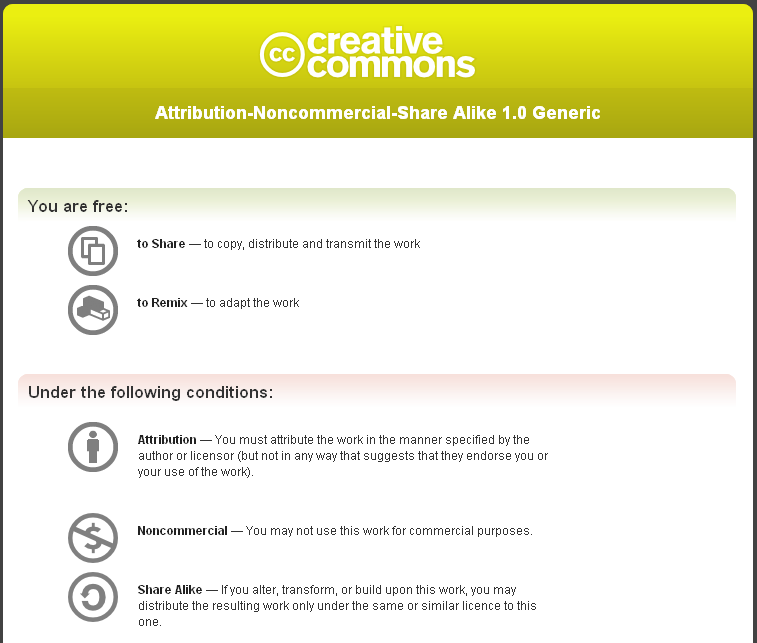
\includegraphics[width=0.50\textwidth]
	{pics/creative_commons.png}
	\caption{\license.}
	\label{fig:testGambar}
\end{figure}


%-----------------------------------------------------------------------------%
\section{Membuat Tabel}
%-----------------------------------------------------------------------------%
Seperti pada gambar, tabel juga dapat diberi label dan caption. Caption pada
tabel terletak pada bagian atas tabel. Contoh tabel sederhana dapat dilihat
pada \tab~\ref{tab:tab1}.

\begin{table}
	\centering
	\caption{Contoh Tabel}
	\label{tab:tab1}
	\begin{tabular}{| l | c r |}
		\hline
		& kol 1 & kol 2 \\
		\hline
		baris 1 & 1 & 2 \\
		baris 2 & 3 & 4 \\
		baris 3 & 5 & 6 \\
		jumlah  & 9 & 12 \\
		\hline
	\end{tabular}
\end{table}

Ada jenis tabel lain yang dapat dibuat dengan \latex~berikut beberapa
diantaranya. Contoh-contoh ini bersumber dari
\url{http://en.wikibooks.org/wiki/LaTeX/Tables}

\begin{table}
	\centering
	\caption{An Example of Rows Spanning Multiple Columns}
	\label{row.spanning}
	\begin{tabular}{|l|l|*{6}{c|}} \hline % create horizontal line
		No & Name & \multicolumn{3}{|c|}{Week 1} & \multicolumn{3}{|c|}{Week 2}
		\\
		\cline{3-8} % create line from 3rd column till 8th column
		& & A & B & C & A & B & C\\
		\hline
		1 & Lala & 1 & 2 & 3 & 4 & 5 & 6\\
		2 & Lili & 1 & 2 & 3 & 4 & 5 & 6\\
		3 & Lulu & 1 & 2 & 3 & 4 & 5 & 6\\
		\hline
	\end{tabular}
\end{table}

\begin{table}
	\centering
	\caption{An Example of Columns Spanning Multiple Rows}
	\label{column.spanning}
	\begin{tabular}{|l|c|l|}
		\hline
		Percobaan & Iterasi & Waktu \\
		\hline
		Pertama & 1 & 0.1 sec \\ \hline
		\multirow{2}{*}{Kedua} & 1 & 0.1 sec \\
		& 3 & 0.15 sec \\
		\hline
		\multirow{3}{*}{Ketiga} & 1 & 0.09 sec \\
		& 2 & 0.16 sec \\
		& 3 & 0.21 sec \\
		\hline
	\end{tabular}
\end{table}

\begin{table}
	\centering
	\caption{An Example of Spanning in Both Directions Simultaneously}
	\label{mix.spanning}
	\begin{tabular}{cc|c|c|c|c|}
		\cline{3-6}
		& & \multicolumn{4}{|c|}{Title} \\ \cline{3-6} & & A & B & C & D \\
		\hline
		\multicolumn{1}{|c|}{\multirow{2}{*}{Type}} & \multicolumn{1}{|c|}{X} &
		1 & 2 & 3 & 4\\ \cline{2-6} \multicolumn{1}{|c|}{}
		& \multicolumn{1}{|c|}{Y} & 0.5 & 1.0 & 1.5 & 2.0\\ \cline{1-6}
		\multicolumn{1}{|c|}{\multirow{2}{*}{Resource}} &
		\multicolumn{1}{|c|}{I} & 10 & 20 & 30 & 40\\ \cline{2-6}
		\multicolumn{1}{|c|}{}                        & \multicolumn{1}{|c|}{J}
		& 5 & 10 & 15 & 20\\ \cline{1-6}
	\end{tabular}
\end{table}


%-----------------------------------------------------------------------------%
\section{Keterkaitan Teori Dengan Penelitian}
%-----------------------------------------------------------------------------%
\todo{Ada baiknya setelah menjelaskan teori-teori, Anda menjelaskan apa kaitan teori tersebut dengan penelitian Anda. Hal ini tentunya membantu pembaca dalam memahami bahwa teori yang Anda paparkan memang penting untuk memahami penelitian Anda nantinya.}

\begin{figure}
	\centering
	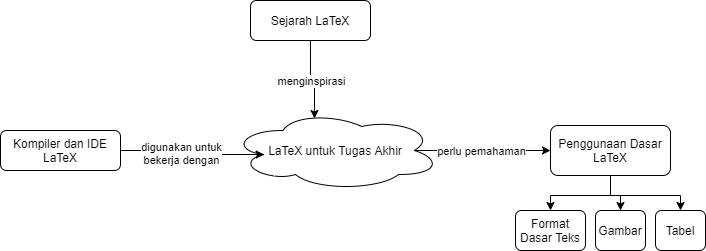
\includegraphics[width=\textwidth]{pics/research_concept_map.png}
	\caption{Keterkaitan konsep hasil studi literatur terhadap penelitian}
	\label{fig:research_concept_map}
\end{figure}

\todo{Jelaskan \pic~\ref{fig:research_concept_map} di sini. Setiap gambar pada
tugas akhir butuh penjelasan. Gambar hadir untuk mempermudah membaca memahami
konteks, tetapi tidak bisa berdiri sendiri tanpa penjelasan. Terkait gambar,
Anda juga bisa mengatur skalanya. Gambar kali ini lebarnya 0,8x dari lebar teks
halaman.}
